% Created 2021-09-23 Thu 12:39
% Intended LaTeX compiler: pdflatex
\documentclass[presentation,aspectratio=169, usenames, dvipsnames]{beamer}
\usepackage[utf8]{inputenc}
\usepackage[T1]{fontenc}
\usepackage{graphicx}
\usepackage{grffile}
\usepackage{longtable}
\usepackage{wrapfig}
\usepackage{rotating}
\usepackage[normalem]{ulem}
\usepackage{amsmath}
\usepackage{textcomp}
\usepackage{amssymb}
\usepackage{capt-of}
\usepackage{hyperref}
\usepackage{khpreamble}
\usepackage{amssymb}
\usepgfplotslibrary{groupplots}
\newcommand*{\shift}{\operatorname{q}}
\definecolor{ppc}{rgb}{0.1,0.1,0.6}
\definecolor{iic}{rgb}{0.6,0.1,0.1}
\definecolor{ddc}{rgb}{0.1,0.6,0.1}
\usetheme{default}
\author{Kjartan Halvorsen}
\date{\today}
\title{Compensator design - Loop shaping}
\hypersetup{
 pdfauthor={Kjartan Halvorsen},
 pdftitle={Compensator design - Loop shaping},
 pdfkeywords={},
 pdfsubject={},
 pdfcreator={Emacs 26.3 (Org mode 9.4.6)}, 
 pdflang={English}}
\begin{document}

\maketitle

\section{Intro}
\label{sec:org3c4ee42}

\section{Lead-lag design}
\label{sec:org86be95f}

\begin{frame}[label={sec:org8d54ba2}]{Specifications on the frequency properties of the closed-loop system}
\begin{center}
\includegraphics[width=0.999\linewidth]{../figures/spec-bode-closed-loop}
\end{center}
\end{frame}

\begin{frame}[label={sec:org6ae2acf}]{The design procedure - overview}
\begin{center}
\fbox{Specifications on the closed-loop system \(G_c(i\omega)\)}\\
\(\downarrow\)\\
\fbox{Specifications on the loop gain \(G_o(i\omega)\)}\\
\(\downarrow\)\\
\fbox{Determine \(F(i\omega)\) in \(G_o(i\omega) = G(i\omega)F(i\omega)\)}\\
\end{center}
\end{frame}

\begin{frame}[label={sec:orgb445bfc}]{From specifications on \(G_c\) to specifications on \(G_o\)}
\begin{center}
\begin{center}
\begin{tabular}{ll}
Closed-loop specifications & Loop gain specifications\\
\hline
Bandwidth \(\omega_B\) & cross-over frequency \(\omega_c\)\\
Resonance peak \(M_p\) & phase margin \(\varphi_m\)\\
Static gain \(G_c(0) \approx 1\) & static gain \(G_o(0)\) high\\
\hline
\end{tabular}
\end{center}
\end{center}


\[ e_0 = |G_c(0)-1| = \left|\frac{G_o(0)}{1+G_o(0)}-1\right| = \left|\frac{1}{1+G_o(0)}\right| < \epsilon\] \[\Rightarrow\]  \[G_o(0) > ?\]
\end{frame}

\begin{frame}[label={sec:org2d3fd3d}]{From specifications on \(G_c\) to specifications on \(G_o\)}
\begin{center}
\begin{center}
\begin{tabular}{ll}
Closed-loop specifications & Loop gain specifications\\
\hline
Bandwidth \(\omega_B\) & cross-over frequency \(\omega_c\)\\
Resonance peak \(M_p\) & phase margin \(\varphi_m\)\\
Static gain \(G_c(0) \approx 1\) & static gain \(G_o(0)\) high\\
\hline
\end{tabular}
\end{center}
\end{center}

\[ e_0 = |G_c(0)-1| = \left|\frac{G_o(0)}{1+G_o(0)}-1\right| = \left|\frac{1}{1+G_o(0)}\right| < \epsilon\] \[\Rightarrow\]  \[G_o(0) > \frac{1}{\epsilon} - 1\]
\end{frame}


\begin{frame}[label={sec:org97e3f19}]{Design procedure in detail}
Given \(G(i\omega)\) and specifications on \(G_o(i\omega)\): \(\omega_c\), \(\varphi_m\), steady-state error \(e_0\).

\begin{center}
\includegraphics[width=1.02\linewidth]{../figures/design-procedure}
\end{center}
\end{frame}


\section{Why lead filter instead of PD controller}
\label{sec:orgde25b4d}
\begin{frame}[label={sec:org1367a19}]{The problem with a PD-controller}
\begin{center}
\begin{tikzpicture}
    \node[anchor=south west,inner sep=0] at (0,0) {\includegraphics[width=0.9\linewidth]{../figures/lead-lag-prep-bode-bode-crop}};
\draw[red,ultra thick,rounded corners] (9.7,2.8) rectangle (12.3,4.5);
\end{tikzpicture} 
\end{center}
\end{frame}

\begin{frame}[label={sec:org4291cdf}]{The problem with a PD-controller, contd}
\begin{center}
  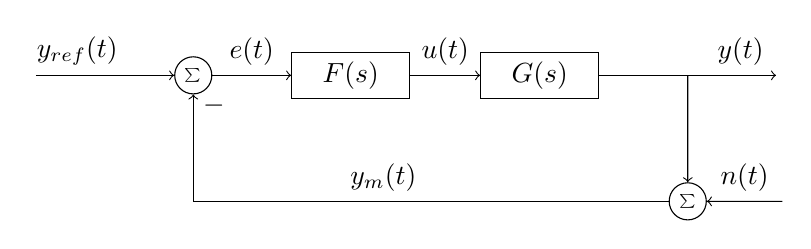
\begin{tikzpicture}[scale = 0.8, node distance=20mm, block/.style={rectangle, draw, minimum width=15mm}, sumnode/.style={circle, draw, inner sep=2pt}]

  \node[coordinate] (refinput) {};
  \node[sumnode, right of=refinput, node distance=20mm] (sumerr) {\tiny $\sum$};
  \node[block, right of=sumerr] (controller) {$F(s)$};
  \node[block, right of=controller, node distance=24mm] (valve) {$G(s)$};
  \node[coordinate, right of=valve, node distance=30mm] (output) {};
  \draw[->] (valve) -- node[coordinate] (measure) {} node[above, pos=0.8] {$y(t)$} (output);
  \node[sumnode, below of=measure, node distance=16mm] (sumnoise) {\tiny $\sum$};
  \node[coordinate, right of=sumnoise, node distance=12mm] (noise) {};

  \draw[->] (refinput) -- node[above, pos=0.3] {$y_{ref}(t)$} (sumerr);
  \draw[->] (sumerr) -- node[above] {$e(t)$} (controller);
  \draw[->] (controller) -- node[above] {$u(t)$} (valve);
  \draw[->] (measure) -- node[above] {} (sumnoise);
  \draw[->] (sumnoise) -| node[above, pos=0.3]{$y_m(t)$} node[right, pos=0.95] {$-$} (sumerr);
  \draw[->] (noise) -- node[above] {$n(t)$} (sumnoise);
  \end{tikzpicture}
\end{center}
\end{frame}




\begin{frame}[label={sec:org8ec2e32}]{The problem with a PD-controller, contd}
\begin{center}
  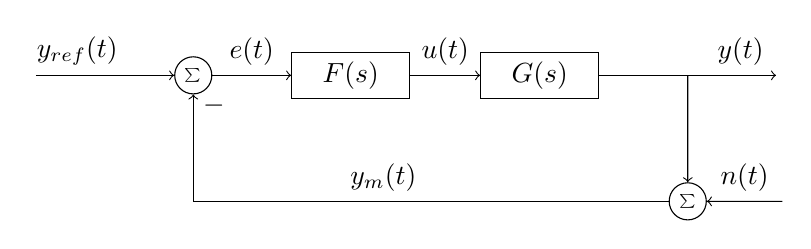
\begin{tikzpicture}[scale = 0.8, node distance=20mm, block/.style={rectangle, draw, minimum width=15mm}, sumnode/.style={circle, draw, inner sep=2pt}]

  \node[coordinate] (refinput) {};
  \node[sumnode, right of=refinput, node distance=20mm] (sumerr) {\tiny $\sum$};
  \node[block, right of=sumerr] (controller) {$F(s)$};
  \node[block, right of=controller, node distance=24mm] (valve) {$G(s)$};
  \node[coordinate, right of=valve, node distance=30mm] (output) {};
  \draw[->] (valve) -- node[coordinate] (measure) {} node[above, pos=0.8] {$y(t)$} (output);
  \node[sumnode, below of=measure, node distance=16mm] (sumnoise) {\tiny $\sum$};
  \node[coordinate, right of=sumnoise, node distance=12mm] (noise) {};

  \draw[->] (refinput) -- node[above, pos=0.3] {$y_{ref}(t)$} (sumerr);
  \draw[->] (sumerr) -- node[above] {$e(t)$} (controller);
  \draw[->] (controller) -- node[above] {$u(t)$} (valve);
  \draw[->] (measure) -- node[above] {} (sumnoise);
  \draw[->] (sumnoise) -| node[above, pos=0.3]{$y_m(t)$} node[right, pos=0.95] {$-$} (sumerr);
  \draw[->] (noise) -- node[above] {$n(t)$} (sumnoise);
  \end{tikzpicture}
\end{center}

\alert{High frequency measurement noise entering the system is amplified in the PD-controller \(F(s)\)}
\end{frame}



\begin{frame}[label={sec:org040c259}]{PD-controller + Low-pass filter = lead compensator + gain}
\begin{center}
  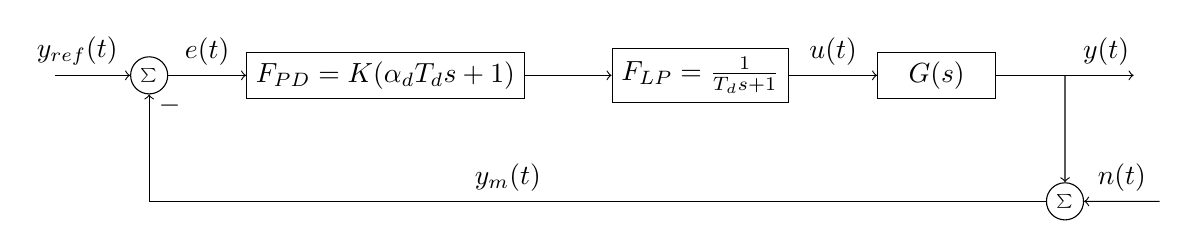
\begin{tikzpicture}[scale = 0.8, node distance=20mm, block/.style={rectangle, draw, minimum width=15mm}, sumnode/.style={circle, draw, inner sep=2pt}]

  \node[coordinate] (refinput) {};
  \node[sumnode, right of=refinput, node distance=12mm] (sumerr) {\tiny $\sum$};
  \node[block, right of=sumerr, node distance=30mm] (controller) {$F_{PD}=K(\alpha_dT_ds + 1)$};
  \node[block, right of=controller, node distance=40mm] (lowpass) {$F_{LP} = \frac{1}{T_ds + 1}$};
  \node[block, right of=lowpass, node distance=30mm] (valve) {$G(s)$};
  \node[coordinate, right of=valve, node distance=25mm] (output) {};
  \draw[->] (valve) -- node[coordinate] (measure) {} node[above, pos=0.8] {$y(t)$} (output);
  \node[sumnode, below of=measure, node distance=16mm] (sumnoise) {\tiny $\sum$};
  \node[coordinate, right of=sumnoise, node distance=12mm] (noise) {};

  \draw[->] (refinput) -- node[above, pos=0.3] {$y_{ref}(t)$} (sumerr);
  \draw[->] (sumerr) -- node[above] {$e(t)$} (controller);
  \draw[->] (controller) -- node[above] {} (lowpass);
  \draw[->] (lowpass) -- node[above] {$u(t)$} (valve);
  \draw[->] (measure) -- node[above] {} (sumnoise);
  \draw[->] (sumnoise) -| node[above, pos=0.3]{$y_m(t)$} node[right, pos=0.95] {$-$} (sumerr);
  \draw[->] (noise) -- node[above] {$n(t)$} (sumnoise);
  \end{tikzpicture}
\end{center}

\(F(s) = KF_{lead} = K \frac{\alpha T_d s + 1}{T_ds + 1}\)
\end{frame}

\begin{frame}[label={sec:org2a0b0e3}]{The lead- and lag filters/compensators}
\begin{center}
\includegraphics[width=0.68\linewidth]{../figures/lead-lag-bode-crop}
\end{center}

\(F_{lead} = \frac{\alpha_d T_d s + 1}{T_ds + 1}, \; \alpha_d > 1  \qquad F_{lag} = \frac{1}{\alpha_i} \cdot \frac{\alpha_i T_i s + 1}{T_is + 1}, \; \alpha_i < 1 \; \text{or}\; F_{lag} = \frac{T_is + 1}{T_is}\)
\end{frame}


\section{Design example}
\label{sec:org6556d7a}

\begin{frame}[label={sec:org485dbfd}]{Position control of a radar antenna}
\begin{center}
\includegraphics[width=0.5\linewidth]{../figures/fig5_1a-crop}
\end{center}
\end{frame}

\begin{frame}[label={sec:orga7c00b7}]{Nyquist plot of the plant}
\begin{center}
\includegraphics[width=0.4\linewidth]{../matlab/5_1-nyqlog-crop}
\end{center}

Will proportional control work? (The open-loop system is stable)
\end{frame}
\end{document}